%! Author = tstreule
%! Date = 18.01.22

\documentclass[%
,a4paper
,fontsize=10pt
,landscape
,pagesize
,headinclude
]{scrartcl}
\usepackage[margin=5mm,headsep=0mm,footskip=4mm]{geometry}

% Preamble and packages
\usepackage{../preamble,../shortcuts}
\usepackage{tikz}
\usetikzlibrary{positioning, shapes}
\graphicspath{{./graphics/}} % Set graphic path
%\usepackage{showframe} % for debugging headers

% >>> [BEGIN] (Re-)formatting >>>
\DeclareDocumentEnvironment{taligned}{+b}{%
    \let\displaystyle\textstyle\aligned#1}{\endaligned}
% <<< [END] (Re-)formatting <<<

% Set title
\title{Deep Learning}
\author{Timo Streule, tstreule@ethz.ch}
\date{\today}

% ======================
% === BEGIN DOCUMENT ===

\begin{document}

    %! Author = tstreule
%! Date = 17.01.22

\thispagestyle{empty} % clear headers and footers
\providecommand\thetitle{LECTURE\_NAME} % ensure a dummy exists

\begin{justify}
\begin{minipage}{.3\textwidth}

    \setmainfont{Noto Serif}
    \KOMAoptions{fontsize=10pt}\color{black}
    \setlength{\parskip}  {0.5em}
    \setlength{\parindent}{1em}

    {\noindent\Large\bfseries Disclaimer}

    This document is an exam summary and follows the given material of the lecture {\itshape \thetitle}.
    Its contribution is a short summary that contains the most important concepts, formulas and algorithms.
    Due to curriculum content updates, some content may not be relevant to future versions of the course.

    I do not guarantee the accuracy or completeness, nor is this document endorsed by the instructors.
    Any errors that are pointed out to me are welcome.
    The complete {\LaTeX} source code can be found at \url{https://github.com/tstreule/eth-cheat-sheets}.

\end{minipage}
\end{justify}

\pagebreak
\pagenumbering{arabic}


    \begin{multicols*}{3}

        % Suppress enumeration of sections
        % \setcounter{secnumdepth}{0}

        \maketitle

        %! Author = tstreule

\section{Connectionism}\label{sec:connectionism}


%% ===
%\subsection{Perceptron}
%
%The perceptron is a symmetric threshold unit:
%\begin{formula}{Sign unit}
%    $\highlight{(\symbf x, \symbf\theta) \mapsto
%    \mathrm{sign}(\symbf x\cdot \symbf\theta)} =
%    \begin{cases}
%        +1 & \textrm{if } \sum_i x_i\theta_i \geq 0 \\
%        -1 & \textrm{otw.}
%    \end{cases}$
%\end{formula}
%
%Given the labels $y = \pm1$, the perceptron starts at $\symbf\theta \leftarrow \symbf 0$ and \textbf{updates} the weights $\symbf\theta \leftarrow \symbf\theta + \Delta\symbf\theta$ only in case of a mistake.
%\begin{formula}{Perceptron rule}
%    $\Delta\symbf\theta =
%    \begin{cases}
%        \symbf 0 & \textrm{if } y \cdot \mathrm{sign}(\symbf{x\cdot\theta}) \geq 0 \\
%        \highlight{y\symbf x} & \textrm{otw.}
%    \end{cases}$
%\end{formula}


% ===
\subsection{Willshaw memory}

Associative memory, pairs of $(\symbf x^t, \symbf y^t) \in \mathcal S$.\quad Learn $\symbf x^t \mapsto \symbf y^t$:
\begin{formula}{W. learning}
    $\begin{cases}
        \highlight{\Theta_{ji} = \min\brace*{
            1, \sum\nolimits_{t=1}^s y_j^t x_i^t
        }}
        \\
        \Theta^t = \symbf y^t (\symbf x^t)^\top
        \:,\quad
        \Theta = \min\brace*{ \symbf 1, \sum\nolimits_{t=1}^s \Theta^t }
    \end{cases}$
\end{formula}

Since $\Theta^t \symbf x^t = (\symbf x^t \cdot \symbf x^t) y^t = ry^t$, retrieving $y$ for a given $\symbf x$ is:
\begin{formula}{W. retrieval}
    $\symbf x \mapsto \symbf z \mapsto \symbf y, \quad
    \highlight{\symbf z = \Theta \symbf x}, \quad
    \highlight{y_j} = \begin{cases} 0 & z_j < r \\ 1 & \textrm{otw.} \end{cases}$
\end{formula}

\begin{figure}[H]
    \centering
    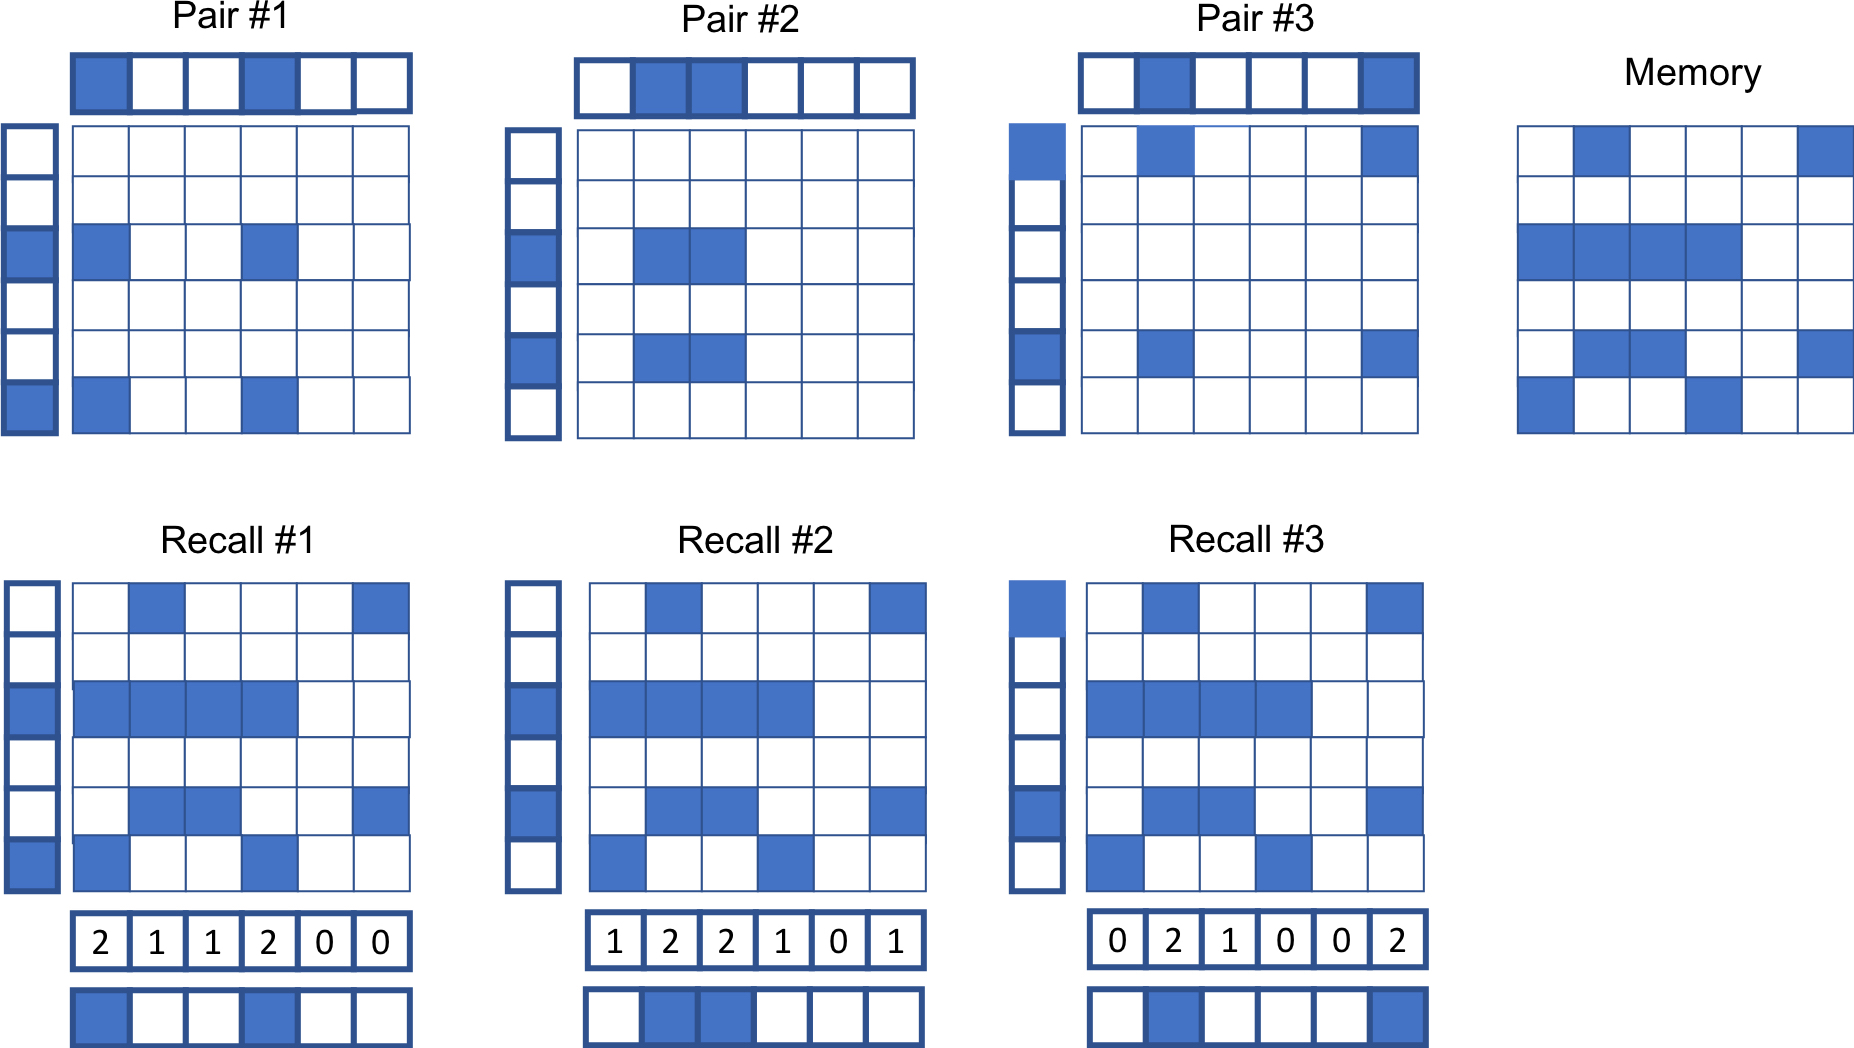
\includegraphics[width=.8\linewidth]{willshaw-memory.jpg}
\end{figure}


% ===
\subsection{Hopfield network}

Assume neurons $x_i \in\brace{-1,1}$ with couplings $\symbf\Theta = (\theta)_{ij}$ such that
\enskip (1) symmetric: \highlight{$\theta_{ij} = \theta_{ji}$}
\enskip (2) irreflexive: \highlight{$\theta_{ii} = 0$}
.

The \textbf{update scheme} is given as follows
\begin{formula}{H. learning}
    $\highlight{x_i \leftarrow \mathrm{sign} \brace*{
        \sum_{j\neq i} \theta_{ij} x_j \green{+ \theta_{i0}}
    }}
    \enspace\green{\text{(bias)}}$
\end{formula}

Convergence is apparent from the Lyapunov equation
\begin{formula}{Ising model}
    $\mathcal E = - \sum\nolimits_{i,j=1}^n \theta_{ij} x_i x_j - \sum\nolimits_{i=1}^n \theta_{i0} x_i$
\end{formula}

Recurr. netw. that can work as \textbf{auto-associative} memory:
\begin{formula}{H. memory}
    $\symbf\Theta \propto \sum\nolimits_{t=1}^s \left[
    \symbf x_t \symbf x_t^\top - \symbf I
    \right] \in \mathbb Z^{n\times n}$
\end{formula}


%% ===
%\subsection{Multilayer perceptron}
%
%\todo{I guess this will come somewhen later...}

        %! Author = tstreule

\section{Linear Networks}\label{sec:linear-networks}

% ===
\subsection{Linear Units}

A linear unit defines a unique direction of change via $\symbf\theta / \norm*{\symbf\theta}$, as well as a constant {\fontspec{Symbola}\symbol{"2639}} rate of change via $\norm*{\symbf\theta}$.
\begin{formula}*{Linear, \green{affine} unit}
    $\iota(\symbf{\tilde x}, \symbf\theta) = \symbf{\tilde x}^\top \symbf\theta \equiv \sum_{i=1}^n x_i \theta_i \green{+ b}$
\end{formula}

Multiple linear units form a \textbf{layer}, resulting in
\begin{formula}{Linear map}
    $L(\symbf x; \symbf\Theta)
    = \brack*{\substack{\textstyle\ldots\smallskip \\ \textstyle\symbf x^\top \symbf\theta^{(j)} \\ \textstyle\smallskip\ldots}}
    = \symbf\Theta \symbf x,
    \enskip \symbf\Theta \in \R^{m\times n}$
\end{formula}

Simple parameter update rule
\begin{formula}{Delta rule}
    $\begin{cases}
        \Delta\symbf\theta = \eta (y - \symbf x^\top \symbf\theta) \symbf x
        \\
        \Delta\symbf\Theta = \eta(\symbf y - \symbf\Theta\symbf x) \symbf x^\top
    \end{cases}$
    \begin{tabular}{c@{}}as simple parameter \\ update rule.\end{tabular}
\end{formula}


% ===
\subsection{Linearity}

A func. $f$ is \textbf{linear \green/ affine}
$\iff f(\alpha \symbf x + \beta \symbf y) = \alpha f(\symbf x) + \beta f(\symbf y) \green + \symbf b$
$\iff f(\symbf x) = \symbf A \symbf x$
\enskip($\forall \symbf x, \symbf y \in \R^n$,\enskip $\forall \alpha, \beta \in \R$,\enskip $\symbf A \in \R^{n\times m}$,\enskip $\green \symbf b \in \R^m$)

\begin{formula}{Composition}
    $f(\symbf x) = \symbf A \symbf x,\ g(\symbf x) = \symbf B \symbf x
    \implies (g \circ f)(x) = \symbf{BAx}$
\end{formula}


% ===
\subsection{Linear Autoencoder}

%Learn compressed data representation, i.e. identity $\symbf{DC\approx I}$.
%Linear AE's aim to learn compressed data representations.
\begin{formula}*{Linear AE}
    $\begin{cases}
        \highlight{\symbf x \overset{\symbf C}{\longmapsto} \symbf z \overset{\symbf D}{\longmapsto} \symbf{\widehat x}},\enskip
        \symbf C,\ \symbf D^\top \in \R^{m\times n},\ m<n
        \\
        \ell(\symbf x) = \frac12 \norm*{\symbf x - \symbf{\widehat x}}^2 = \frac12 \norm*{\symbf x - \symbf{DCx}}^2
    \end{cases}$
\end{formula}

\begin{formula}*{Auto-loss}
    $(\symbf{C^\ast,D^\ast}) \xleftarrow{\hphantom{\arg\min}}\mathllap{\substack{\arg\min\\~\\~}\mkern6mu} \frac{1}{2s} \sum_{t=1}^s \ell(\symbf x_t) = \frac12 \norm*{\symbf X - \symbf{DCX}}_F^2$\\
    with \textbf{Frobenius norm} $\norm*{\symbf A}_F \coloneqq \sqrt{\sum_{i,j} \abs{a_{ij}}^2}$
\end{formula}

The \textbf{goal} is to learn the identity $\symbf{DC} \approx \symbf I$ via the \textbf{AE gradients}
\begin{formula}
    $\pderiv{\ell(\symbf x)}{\symbf C} = \symbf D^\top (\symbf{\widehat x} - \symbf x) \symbf x^\top \gray \in \R^{m\times n}$,\enskip
    $\pderiv{\ell(\symbf x)}{\symbf D} = (\symbf{\widehat x} - \symbf x) \symbf x^\top \symbf C^\top \gray \in \R^{n\times m}$
\end{formula}

\begin{formula}{Eckard-Young}
    Choose $\symbf D = \symbf U_k$ and $\symbf C = \symbf U_k^\top$ given $\symbf X = \symbf{U\Sigma V^\top}$ (not unique!)
\end{formula}

\begin{formula}{Reduced~~~\\rank}
    $\rank(\symbf{DC}) \leq \min \brace*{\rank(\symbf C),\ \rank(\symbf D)} \leq m < n$
    \\
    $\gray\symbf{\widehat X} = \symbf{DCX}$,\enskip $\rank(\symbf {\widehat X}) \leq \min\brace*{m,\ \rank(\symbf X)} \leq m$
\end{formula}


% ===
\subsection{Deep Linear Gradients}

\todo

        %! Author = tstreule

\section{Sigmoid Networks}\label{sec:sigmoid}


Composition of linear unit w/ non-linear \orange{activation function}.
\begin{formula}*{Ridge unit}
    $f = \orange{\phi} \circ \iota,\enskip f(\symbf x; \symbf\theta) = \orange{\phi}(\symbf x^\top \symbf\theta)$
\end{formula}

For any loss function $\ell$, the parameter updates read
\begin{formula}{Updates}
    $\nabla_{\symbf\theta} (\ell \circ \phi)(\symbf x^\top \symbf\theta)
    = (\mathcal L \circ \phi)'(\symbf x^\top \symbf\theta)
    \underbracket{\ \symbf x\ }_{\mathllap{\text{direction fully determined by}\ \symbf x}\ \hookleftarrow}$
\end{formula}


% ===
\subsection{Threshold units \enskip\mdseries(not differentiable)}

\begin{formula}{Sign unit \& Heavyside}
    $\highlight{\sign(\symbf x^\top \symbf\theta)} \gray \in \brace{-1,1}$,\enskip
    $H(z) \gray \in \brace{0,1}$
\end{formula}

The perceptron is a symmetric threshold unit.
\begin{formula}*{Perceptron}
    $\highlight*{\ell(\symbf x, y; \symbf\theta)} = \min\brace{0,\ y \symbf{x^\top\theta}} = \max\brace{0,\ -y \symbf{x^\top\theta}}$,\\
    $\highlight{\nabla_{\symbf\theta}\ell (\symbf x, y; \symbf\theta)} \equiv \Delta\symbf\theta =
    \begin{cases}
        \symbf0 & y\symbf{x^\top\theta} \geq 0\\
        y \symbf x & \text{otw.}
    \end{cases}$
\end{formula}
Given the labels $y = \pm1$, the perceptron starts at $\symbf\theta \leftarrow \symbf 0$ and \textbf{updates} the weights $\symbf\theta \leftarrow \symbf\theta + \Delta\symbf\theta$ only in case of a mistake.


% ===
\subsection{Logistic unit \enskip\mdseries($C^\infty$ smooth \& monotone)}

\begin{formula}*{Sigmoid}
    $\highlight*{\sigma(z)} = \dfrac{1}{1 + \eu^{-z}} = \dfrac{\eu^z}{\eu^z + 1}$\enskip
    $\gray \in [0,1]$,\quad $z \coloneqq \symbf{x^\top\theta}$
\end{formula}
\begin{formula}
    $\highlight{\sigma'(z)} = \sigma(z)(1 - \sigma(z)) = \sigma(z) \sigma(-z)$,\quad
    $\highlight{\sigma^{-1}(z)} = \ln \dfrac{z}{1 - z}$
\end{formula}

\begin{formula}*{Hyperbolic}
    $\highlight*{\tanh(z)} = \dfrac{\eu^z - \eu^{-z}}{\eu^z + \eu^{-z}} = 2 \sigma(2z) - 1$\enskip
    $\gray \in [\shortminus1,1]$
\end{formula}
\begin{formula}
    $\tanh(z) = \frac{2\sinh(z)}{2\cosh(z)}$,\quad
    $\highlight{\nabla_z\tanh(z)} = 1 - \tanh^2(z)$%,\quad
%    $\tanh^{\shortminus1} (z) = \frac12 [\ln(1+z) - \ln(1-z)]$
\end{formula}


\subsubsection{Softmax \enskip\mdseries($k$ classes)}

\begin{formula}*{Softmax}
    $\highlight*{\sigma_i\ap{max} (z_i)} = \dfrac{\exp*(z_i)}{\sum_{j=1}^k \exp*(z_j)}$,\quad
    $z_i \coloneqq \symbf{x^\top\theta}_i$
\end{formula}

We recover the sigmoid for $k=2$:
\begin{formula}
    $\text{soft-max w/}\ \symbf\theta_1, \symbf\theta_2 \iff \text{sigmoid w/}\ \symbf\theta \coloneqq \symbf\theta_1 - \symbf\theta_2$
\end{formula}


\subsubsection{Cross-entropy loss}

\begin{formula}{Probability}
    $\highlight{\P{Y=y \mid \symbf x \gray ; \symbf\theta}} = \sigma(yz)$,\quad $z = \symbf{x^\top\theta}$
\end{formula}

\begin{formula}*{Binary CE}
    $\highlight*{\ell(\symbf x, y; \symbf\theta)} = - \ln \sigma(y \symbf{x^\top\theta}))$\hfill for $y \in \brace{\shortminus1,1}$\\
    $\ldots = -y \ln \sigma(z) - (1\shortminus y) \ln (1 \shortminus \sigma(z))$\hfill for $y \in \brace{0, 1}$\\
$\highlight{-\nabla_{\symbf\theta} \ell(\symbf x, y; \symbf\theta)} = \sigma(-yz) y \cdot \symbf x$
\end{formula}

\begin{formula}*{Softmax CE}
    $\begin{taligned}[t]
        \highlight*{\ell(\symbf x, \symbf y; \symbf\Theta)} &= -\symbf y \cdot \ln \sigma\ap{max} (\symbf x; \symbf\Theta)\\
        &= -\sum_{i=1}^k y_i \symbf{x^\top\theta}_i + \underbracket{\ln\paren*{\sum_i \exp*(\symbf{x^\top\theta}_i)}}_{\text{norm. constant}}
    \end{taligned}$\\[-.8em]
    $\highlight{\nabla_{\symbf\theta_i} \ell (\symbf x, \symbf y; \symbf\Theta)} = (\sigma_i\ap{max} - y_i) \cdot \symbf x$
\end{formula}


% ===
\subsection{Multilayer perceptron (MLP)}


\begin{figure}[H]
    \centering
    \scalebox{.75}{%! Credits: https://latexdraw.com/drawing-neural-networks-in-tikz-short-guide/

\begin{tikzpicture}[
    >=stealth, % default arrow style
]

% Input layer neurons'number
    \newcommand{\inputnum}{3}
% Hidden layer neurons'number
    \newcommand{\hiddennum}{3}
% Output layer neurons'number
    \newcommand{\outputnum}{2}
% Node size
    \newcommand{\nodesize}{1.5em}
% Vertical/horizontal shifts
    \newcommand{\vnodeshift}{2.5em}
    \newcommand{\hnodeshift}{8em}
% Colors
    \colorlet{input-layer-color}{orange!30}
    \colorlet{hidden-layer-color}{teal!30}
    \colorlet{output-layer-color}{purple!30}

% Input Layer
    \foreach \i in {1,...,\inputnum}{
        \node[circle,
            minimum size = \nodesize,
            fill=input-layer-color,
        ] (Input-\i) at (0,-\i*\vnodeshift) {};
    }
%    \node[below = 0cm and 0cm of Input-\inputnum] {$\symbf x \in \R^n$};

% Hidden Layer
    \foreach \i in {1,...,\hiddennum}{
        \node[circle,
        minimum size = \nodesize,
        fill=hidden-layer-color,
        yshift=(\hiddennum-\inputnum)*\nodesize
        ] (Hidden-\i) at (1*\hnodeshift,-\i*\vnodeshift) {};
    }

% Output Layer
    \foreach \i in {1,...,\outputnum}{
        \node[circle,
        minimum size = \nodesize,
        fill=output-layer-color,
        yshift=(\outputnum-\inputnum)*\nodesize
        ]  (Output-\i) at (2*\hnodeshift,-\i*\vnodeshift) {};
    }
%    \node[below = 0cm and 0cm of Output-\outputnum] {$\symbf y \in \R^l$};

% Connect neurons In-Hidden
    \foreach \i in {1,...,\inputnum}{
        \foreach \j in {1,...,\hiddennum}{
            \ifthenelse{\equal{\j}{1}}{%
                \ifthenelse{\equal{\i}{1}}{%
                    \draw[->, shorten >=1pt, thick] (Input-\i)
                    --node[above]{$\symbf\theta_{\j} \in \R^{n}$} (Hidden-\j);
                }{%
                    \draw[->, shorten >=1pt, thick] (Input-\i) -- (Hidden-\j);
                }
            }{%
                \draw[->, shorten >=1pt] (Input-\i) -- (Hidden-\j);
            }
        }}

% Connect neurons Hidden-Out
    \foreach \i in {1,...,\hiddennum}{
        \foreach \j in {1,...,\outputnum}{
            \ifthenelse{\equal{\j}{1}}{%
                \ifthenelse{\equal{\i}{1}}{%
                    \draw[->, shorten >=1pt, thick] (Hidden-\i)
                    --node[above]{$\symbf\beta_\j \in \R^{m}$} (Output-\j);
                }{%
                    \draw[->, shorten >=1pt, thick] (Hidden-\i) -- (Output-\j);
                }
            }{%
                \draw[->, shorten >=1pt] (Hidden-\i) -- (Output-\j);
            }
        }}

% Inputs
    \foreach \i in {1,...,\inputnum}{
        \draw[stealth-, shorten <=1pt] (Input-\i) -- ++(-.33*\hnodeshift,0) node[left]{$x_{\i}$};
    }

% Outputs
    \foreach \i in {1,...,\outputnum}{
        \draw[->, shorten >=1pt] (Output-\i) -- ++(.33*\hnodeshift,0) node[right]{$y_{\i}$};
    }

% --- Summarized MLP ---

    \node[circle,
        minimum size = \nodesize,
        fill=input-layer-color,
    ] (Input) at (0,-4*\vnodeshift-1em) {};
    \node[above = 0cm and 0cm of Input] {$\mathllap{\gray\R^n \ni\ } \symbf x$};

    \node[circle,
        minimum size = \nodesize,
        fill=hidden-layer-color,
    ] (Hidden) at (\hnodeshift,-4*\vnodeshift-1em) {};
    \node[above = 0cm and 0cm of Hidden] {$F_{\symbf\theta} \circ \symbf x$};

    \node[circle,
        minimum size = \nodesize,
        fill=output-layer-color,
    ] (Output) at (2*\hnodeshift,-4*\vnodeshift-1em) {};
    \node[above = 0cm and 0cm of Output] {$G_{\symbf\beta} \circ F_{\symbf\theta} \circ \symbf x \mathrlap{\gray\ \in \R^l}$};

    \draw[stealth-, shorten <=1pt] (Input) -- ++(-.33*\hnodeshift,0);
    \draw[->, shorten >=1pt] (Input) --node[]{\highlight{$\symbf\theta$}} (Hidden);
    \draw[->, shorten >=1pt] (Hidden) --node[]{\highlight{$\symbf\beta$}} (Output);
    \draw[->, shorten >=1pt] (Output) -- ++(.33*\hnodeshift,0);

\end{tikzpicture}
}
\end{figure}

\begin{formula}{Forward}
    $y_k \equiv f_k(\symbf{x; \beta, \theta}) = \sum_{j=1}^m \beta_{kj}\ \sigma(\symbf\theta_j^\top \symbf x) = \symbf{\beta}_k^\top \sigma(\symbf\Theta \symbf x)$
\end{formula}
\begin{formula}{Backw. (SGD)}
    $\theta \leftarrow \theta - \eta \cdot \displaystyle \pderiv{\frac12(f(\symbf x) - y)^2}{\theta}$,\quad
    $\theta \in \brace{\beta_j, \theta_{ji}}$,\enskip $\eta > 0$
\end{formula}

        %! Author = tstreule

\section{Approximation Theory}\label{sec:approximation-theory}


% ===
\subsection{Universality}

\begin{formula}{Weierstrass\\Theorem}
    Polynomials $\mathcal P$ are \textbf{dense} in $C(I)$, \textit{i.e.} set of intervals, where $I = [a, b]$ for any $a<b$.
    \\\llap{\textit{w.l.o.g.:}\enskip}%
    Assume $I = [0, 1]$ \& define $\phi : C(I) \mapsto C([a, b])$,\enskip $\phi(f) = f\circ\phi$,\enskip $\phi = (1 - t)a + tb$.
\end{formula}

\begin{highlightbox}
    An MLP $\mathcal H_\sigma^n$ with any continuous, \textit{non}-polynomial activation function $\sigma \in C^\infty(\R^n)$ is a universal approximator.
    \begin{equation*}
        \mathcal G_\sigma^n = \brace{g : g(\symbf x) = \sigma(\symbf{\theta^\top x}) \mid \symbf\theta \in \R^n},\quad
        \mathcal H_\sigma^n = \mathop{\mathrm{span}}(\mathcal G_\sigma^n)
    \end{equation*}
\end{highlightbox}


% ===
\subsection{Complexity}

Universality is the rule not the exception but at what cost? Deeper networks may yield better approximations but there's no evidence for/against it.
\begin{itemize}
    \item \textit{MLPs do not suffer from the curse of dimensionality} when approximating func. $g$ with $C_g \coloneqq \int \norm{\omega} \abs{\hat g(\omega)} \diff\omega < \infty$.
    \item approx. error rate $\propto 1/m$ ($m = \text{\#units}$)
\end{itemize}

        %! Author = tstreule

\section{Backpropagation}\label{sec:backpropagation}


\begin{formula}
    \bfseries\setstretch{0.9}
    \renewcommand{\labelenumi}{\normalfont\scriptsize\arabic{enumi}:}
    \begin{enumerate}[leftmargin=1.5em,labelsep=0.5em]
        \item $\symbf z_0 = \symbf x$ \gray{\normalfont\cdotfill$\vartriangleright$ Forward pass\enskip~}
        \item for $l=1{\ldots}k$ do
        \item \quad $\symbf z_l = F_l(\symbf z_{l-1})$
        \item end for
        \item $\symbf\xi_{k+1} = \partial\ell(\symbf z_k)$ \gray{\normalfont\cdotfill$\vartriangleright$ Backward pass\enskip~}
        \item for $l=k{\ldots}1$
        \item \quad $\symbf\xi_l = \symbf\xi_{l+1} \cdot \partial F_l(\symbf z_{l-1})$
        \item end for
        \item for $l=1{\ldots}k$ do \gray{\normalfont\cdotfill$\vartriangleright$ Local computations\enskip~}
        \item \quad $\nabla_l = \symbf\xi_{l+1} \cdot F_l'(\symbf z_{l-1})$
        \item end for
    \end{enumerate}
\end{formula}
%\begin{formula}
%    \bfseries
%    \renewcommand{\labelenumi}{\normalfont\scriptsize\arabic{enumi}:}
%    \begin{enumerate}[leftmargin=1.5em,labelsep=0.5em]
%        \item $\symbf z[0] = \symbf x$ \gray{\normalfont\cdotfill$\vartriangleright$ Forward pass\enskip~}
%        \item for $l=1{\ldots}k$ do
%        \item \quad $\symbf z[l] = F_l(\symbf z[l-1])$
%        \item end for
%        \item $\symbf\xi[k+1] = \partial\ell(\symbf z[k])$ \gray{\normalfont\cdotfill$\vartriangleright$ Backward pass\enskip~}
%        \item for $l=k{\ldots}1$
%        \item \quad $\symbf\xi[l] = \symbf\xi[l+1] \cdot \partial F_l(\symbf z[l-1])$
%        \item end for
%        \item for $l=1{\ldots}k$ do \gray{\normalfont\cdotfill$\vartriangleright$ Local computations\enskip~}
%        \item \quad $\nabla[l] = \symbf\xi[l+1] \cdot F_l'(\symbf z[l-1])$
%        \item end for
%    \end{enumerate}
%\end{formula}


% ===
\subsection{Layers}

\begin{formula}{DAG}
    Directed Acyclic Graphs represent connectivity structure between computational units.
\end{formula}

In DNNs typically units are arranged in sequence of \textbf{layers}
\begin{formula}{Composition}
    $F = F_{\orange k:1} = F_{\orange k} \circ\cdots\circ F_{\orange 1}$\\
    $\mathrm{width}_l \equiv n_l \coloneqq \mathrm{dim}(\mathrm{range}(F_l))$,\enskip $\mathrm{\#units} = \sum_{l=1}^k n_l$
\end{formula}

Such layer-to-layer maps successively tansform input into intermediate representations
\begin{formula}*{Activation}
    \highlight{$\symbf z_l \coloneqq F_{l:1}(\symbf x) = (F_l \circ F_{l-1:1})(\symbf x) = F_l(\symbf z_{l-1})$}\\
    $\symbf z_0 \coloneqq \symbf x$: input layer,\quad $\symbf y \eqqcolon \symbf z_k$: output layer
\end{formula}


% ===
\subsection{Multivariate analysis}

\begin{formula}{Chain rule}
    $\partial (g \circ f) = (\partial g \circ f) \cdot f$ \enskip generalized to maps\\
    $\mathllap{\gray \partial F_{g:f} \equiv\ } \highlight{\partial(F_g \circ F_f) = (\partial F_g \circ F_f) \cdot \partial F_f}$
    \begin{formula}*{for DNNs}
        $\highlight*{\partial F_{l:1} = \prod_{l=k}^1 \partial F_l \circ F_{l-1:1}}$
    \end{formula}
\end{formula}

\begin{formula}{Notation}
    $F \colon \R^n \times \R^d \to \R^m$, inputs $\symbf x \in \R^n$, parameters $\symbf\theta \in \R^d$\\
    $\partial f = \paren*{\displaystyle\pderiv{f}{x_i}}_{\mkern-5mui} \mkern-4mu \green{\! \overset{m=1}{=} \!} \partial F = \paren*{\displaystyle\pderiv{F_j}{x_i}}_{\mkern-5muji} \mkern-4mu$,\enskip $f' = \nabla_\theta f$,\enskip $F' = \nabla_\theta F$
\end{formula}


% ===
\subsection{Gradient descent}

For learning we're not interested in prediction $F$, but in loss $f$
\begin{formula}{Loss}
    $\highlight{f \coloneqq \ell \circ F = \ell \circ F_{k:1}} = \ell(F(\symbf{x,\theta}), \symbf y)$,\quad $\ell : \mathcal Y \times \mathcal Y \to \R$
\end{formula}
The (normalized) \textbf{negative gradient} $\propto - \nabla_\theta f(\symbf{x,\theta})$ will define the direction of the steepest descent on the loss.

\begin{formula}{\orange\warning}
    There exist two different gradients w.r.t. maps $F_l$, \textit{input/activity} and \textit{\bfseries parameters}. Don't be confused!
\end{formula}

\begin{formula}*{Gradient}
    \highlight*{$\nabla_{\orange\symbf\theta_l} F = (\partial F_{k:l+1} \circ F_{l:1}) \cdot (F_l' \circ F_{l-1:1})$} $(\forall l)$\\
    $\nabla_{\orange\symbf\theta_l} f (\symbf x) = \underbrace{\partial (\ell \circ F_{k:l+1}) (\symbf z_l)}_{\mathclap{\symbf\xi_{k+1} \colon \text{downstream}}} \enskip\cdot\enskip \underbrace{F_l' (\symbf z_{l-1})}_{\mathclap{\text{local Jacob.}\mathrlap{\text{\ \ $(\symbf z_{l-1}$: upstream)}}}}$
\end{formula}

\begin{formula}{vector-Jacobian product}
    for \enskip $\symbf z = \symbf{W x}$ \enskip we find \highlight{$\pderiv{\symbf z}{\symbf W} = \symbf x^\top$}
\end{formula}


% ===
\subsection{Parameter gradients}

\begin{formula}{Ridge function layer}
    $\nabla_{\symbf\theta_{lj}} \ell(\symbf x) = \underbrace{\xi_{lj}}_{\mathclap{\text{Scalar}}} \enskip\cdot\enskip \underbrace{\sigma' (\symbf\theta_{lj} \cdot \symbf z_{l-1})}_{\mathclap{\text{Sensitivity of unit}}} \enskip\cdot\enskip \underbrace{\symbf z_{l-1\vphantom{j}}}_{\mathclap{\text{Direction}}}$
\end{formula}
\begin{formula}{Deep lin. netw.}
    $F(\symbf x) = \prod_{l=k}^1 \symbf\theta_l \symbf x$,\quad $f = \ell \circ F$
\end{formula}
\begin{formula}
    $\highlight{\partial F_l} = \symbf\theta_l$,\quad $\partial F_{k:l} = \prod_{r=k}^l \symbf\theta_r$,\quad
    $\highlight{\symbf\xi_k} = \nabla \ell(\symbf z_k)$,\quad $\symbf\xi_{l-1} = \symbf\xi_l \symbf\theta_l$\\
    $\highlight{\nabla_{\orange \symbf\theta_l} f(\symbf x)} =
    \begin{bmatrix}
        \symbf\theta_k & \ldots & \orange{\symbf\theta_{l+1}} & \delta
    \end{bmatrix}
    \begin{bmatrix}
        \orange{\symbf\theta_{l-1}} & \ldots & \symbf\theta_1 & \symbf x
    \end{bmatrix}^{\top}
    = \symbf\xi_l \symbf z_{l-1}^\top$
\end{formula}

        %! Author = tstreule

\section{Rectified Networks}\label{sec:rectified-networks}


% ===
\subsection{Rectified linear unit --- ReLU}

\begin{formula}*{ReLU}
    $\highlight*{(\symbf{x, \theta})_{\orange\boldsymbol+}} \coloneqq \max\brace{0, \symbf{x \cdot \theta}}$,\quad
    $\partial (z)_{+} =
    \begin{cases}
        1 & \text{if } z>0 \\
        0 & \text{if } z<0
    \end{cases}$
\end{formula}
\begin{itemize}
    \item backprop very simple: gradient either $0$ or the weight value
    \item sparseness of Jacobi matrix can be exploited
    \begin{formula}
        $\partial F_l = \symbf{\tilde\Theta} \coloneqq \paren*{\symbf{\tilde\theta}_{li}^\top}_i$,\quad
        $\symbf{\tilde\theta}_{ij} =
        \begin{cases}
            \symbf0 & \text{if } z_{lj}=0 \\
            \symbf\theta_{lj} & \text{otw.}\quad\leftarrow\ \text{weight value!}
        \end{cases}$
    \end{formula}
    \item can lead to dying \textit{(inactive)} ReLU
\end{itemize}


% ===
\subsection{Absolute value unit --- AbsU}

\begin{formula}{AbsU}
    $\partial\abs{z} =
    \begin{cases}
        1 & z>0 \\
        \shortminus1 & z<0
    \end{cases}$,\enskip
    \highlight{$(z)_+\! = \frac{z + \abs{z}}{2}$} and \highlight{$\abs{z} = 2(z)_+\! - z$}
\end{formula}


% ===
\subsection{Smooth ReLU approximations}

\begin{tabular}{@{}>{\bfseries}l<{:}l@{}}
    Softplus & $\sigma\ap{softp}(z) = \log(1 + \eu^z)$\\
    Exp. LU & $\sigma\ap{expLU}(z) =
    \begin{cases}
        z & z \geq 0 \\
        \eu^z - 1 & \text{otw.}
    \end{cases}$\\
    Leaky ReLU & $\sigma\ap{\ell ReLU}(z) =
    \begin{cases}
        z & z \geq 0 \\
        \epsilon \cdot z & \text{otw.}
    \end{cases}$
\end{tabular}


% ===
\subsection{Piecewise linear approximation}

\begin{formula}{Theorem}
    Piecewise linear functions are \textit{dense} in $C([0;1])$.
\end{formula}

\begin{formula}
    with $m$ pieces:\quad
    $g(x) = \underbrace{ax + b}_{\text{linear}} \enskip+\enskip \underbrace{\sum_{i=1}^{m-1} c_i (x - x_i)_{\orange+}}_{\mathclap{\text{changes of slope, but \textit{no} shift}}}$
\end{formula}


% ===
\subsection{Hinge functions}

2+ hyperplanes glued together: $g(\symbf x) = \max(\symbf\theta_1 \symbf x + b_1,\ \symbf\theta_2 \symbf x + b_2)$


% ===
\subsection{Polyhedral functions}

\begin{formula}{Polyhedral}
    $f$ is \textit{polyhedral} $\iff$ $\mathrm{epi(f)}$ is a polyhedral set\\
    Epigraph: $\mathrm{epi(f)} \coloneqq \brace{(\symbf x, t) \in \R^{n+1} \colon f(\symbf x) \leq t}$
\end{formula}

\begin{formula}
    A \textit{set} $S$ is polyhedral $\iff$ $S = \brace{\symbf x \in \R^n \colon \symbf\theta_j \symbf x + b_j \geq 0, j=1,{\ldots},r}$\\
    \gray{$\to$ finite \#hyperplanes sufficient to approximate a polyh. set}
\end{formula}

\begin{formula}*{Thm.}
    Every continuous pieccewise linear function $f$ can be written as the difference of \textbf{two} polyhedral functions. $f(\symbf x) = \max\limits_{(\symbf\theta, b) \in \mathcal A^+} \brace{\symbf{\theta x} + b} -  \max\limits_{(\symbf w, b) \in \mathcal A^-} \brace{\symbf{w x} + b}$
\end{formula}

        %! Author = tstreule

\section{Optimization}\label{sec:optimization}


% ===
\subsection{Objectives}

\begin{formula}{Squared loss}
    \highlight{$\ell_{\symbf y} (\symbf\nu) = \frac12 \norm{\symbf{y - \nu}^2}$}
\end{formula}
\begin{formula}{Classification loss}
    $\ell_{y} (\nu) =
    \begin{cases}
        0 & \text{if } \nu = y \\
        1 & \text{otw.}
    \end{cases}$\quad (has no gradients)
\end{formula}

\begin{formula}{Probabilistic loss}
    \highlight{$\ell_{\symbf y} (\symbf\nu) = - \log p(\symbf{y; \nu})$}
\end{formula}
\begin{itemize}
    \item \textbf{Gaussian models:}\enskip
    $p(\symbf{y; \nu}) = \prod_{j = 1}^m \frac{1}{\sqrt{2\pi}} \exp*(- \frac12 (y_j - \nu_j))^2$ \\
    $\implies \ell_{\symbf y} (\symbf\nu) = \frac12 \norm{\symbf{y - \nu}}^2 + \const$
    \item \textbf{Exponential:}\enskip
    $p(\symbf{y; \nu}) = \cancel{h(\symbf y)} \exp(\symbf{y \nu} - \phi(\symbf\nu))$ \\
    $\implies \ell_{\symbf y} (\symbf\nu) = - \symbf{y \nu} + \phi(\symbf\nu) + \const$
    \item \textbf{Poisson models:}\enskip
    $p(y; \nu) = \nu^y \frac{\eu^{-\nu}}{y!}$ \\
    $\implies \ell_y (\nu) = \nu - y \log \nu + \const$,\enskip $\nu > 0$
\end{itemize}


% ===
\subsection{Expected vs. empirical risk}

\begin{formula}{Expected}
    $\mathcal R (\symbf\theta) = \E[(\symbf{x,y})]{\ell (F(\symbf{x; \theta}))}
    \implies
    \highlight{\symbf\theta^\ast = \arg\min_{\symbf\theta} \mathcal R(\symbf\theta)}$
\end{formula}

\begin{formula}{Empirical}
    $\hat{\mathcal R} (\symbf\theta) = \frac1s \sum_{t=1}^s \ell_{\symbf y^t} \paren*{F(\symbf x^t; \symbf\theta)}$
\end{formula}


% ===
\subsection{Gradient descent --- GD}

Use Taylor approx. $f(\symbf x + \Delta\symbf x) \approx g(\symbf x)$ and set $\nabla g(x) \overset!= 0$.

\begin{formula}{$\implies$ Newton's method}
    \highlight{$\Delta \symbf x = - \orange{[\nabla^2 f(\symbf x)]^{-1}} \nabla f(\symbf x)$}
\end{formula}

Idea: Find matrix $\symbf B$ close to the Hessian, i.e. $\norm{\nabla^2 f(\symbf x) - \symbf B}_2 \leq \epsilon$

\begin{formula}*{Gradient descent}
    Assuming $\nabla^2 f(\symbf x) = \frac1\eta \symbf I$, we recover\\
    \highlight{$\Delta\symbf x = - \eta \nabla f(\symbf x)$},\enskip step size $\eta > 0$
\end{formula}

\begin{formula}*{Gradient flow}
    \highlight{$\dot{\symbf x} = - \nabla f(\symbf x)$},\enskip grad. descent with $\eta \to 0$
\end{formula}


\subsubsection{Optimal learning rate}

Start w/ convex quadratic objective $f(\symbf x) = \frac12 \symbf{x^\top Q x} - \symbf{q x}$ with $\symbf Q = \symbf{\orange{U} \Lambda \orange{U}^\top}$ p.s.d., thus $f$ convex.
Change the basis as $\symbf x \leftarrow \symbf{U^\top}$ and $\symbf q \leftarrow \symbf{U^\top q}$ and effectively minimize the \textit{separable} problem: $f(\symbf x) = \sum_{i=1}^n g_i (x_i)$,\enskip $g_i(z) = \frac{\lambda_i}{2} z^2 - q_i z$,\enskip $\lambda_i > 0$.

\begin{formula}{Exp. convergence if}
    $\eta < \frac2\lambda$ (1-dim.),\quad
    $\eta \leq \frac{2}{\lambda\ped{max} (\symbf Q)}$ (n-dim.)
\end{formula}
\begin{formula}{Optimal}
    $\highlight{\eta^\ast} = \min\limits_\eta \max \brace{\eta\lambda\ped{max} \!- 1,\ 1 - \eta\lambda\ped{min}} = \highlight{\frac{2}{\lambda\ped{max} + \lambda\ped{min}}}$
\end{formula}


\subsubsection{Convexity}

\begin{formula}{$L$-smooth function}
    $\norm{\nabla f(\symbf x) - \nabla f(\symbf x + \Delta\symbf x)} \leq L \norm{\Delta\symbf x}$ \\
    \llap{\gray$C^{2} \rightsquigarrow\ $}$f(\symbf x + \Delta\symbf x) \leq f(\symbf x) + \nabla f(\symbf x) \cdot \Delta\symbf x + \frac{L}{2} \norm{\Delta\symbf x}^2$
\end{formula}
\begin{formula}{$\mu$-strongly convex}
    $f(\symbf x + \Delta\symbf x) \geq f(\symbf x) + \nabla f(\symbf x) \cdot \Delta\symbf x + \frac\mu2 \norm{\Delta\symbf x}^2$ \\
    \gray Convex if $\mu = 0$.
\end{formula}
$\implies$ Can be sandwiched: $\mu \symbf I \preceq \nabla^2 f \preceq L \symbf I$

\todo{Lec. ch08-a: slide 26-39}

\begin{formula}{Convexity}
    $\ell(\lambda w + (1 - \lambda) w') \leq \lambda \ell(w) + (1 - \lambda) \ell(w')$\\
    $\iff \ell(w) \geq \ell(w') + \nabla \ell(w')^\top (w - w')$
\end{formula}
Given also \textbf{$\symbfit L$-smoothness}, i.e. $\norm{\nabla \ell(w) - \nabla \ell(w')} \leq L \norm{w - w'}$, then $\implies \ell(w) \leq \ell(w') + \nabla \ell(w')^\top (w - w') + \frac{L}{2} \norm{w - w'}^2$.


% ===
\subsection{Stochastic gradient descent --- SGD}

Approximate true gradient with mean gradient of batch. Sacrifice statistical efficiency at benefit of reduced variance.

\begin{formula}{Unbiased}
    $\E{\nabla f_I(\symbf x)} = \sum_{i=1}^n \frac1n \nabla f_i (\symbf x) = \nabla f(\symbf x)$
\end{formula}
\begin{formula}{Variance}
    $\V{\symbf x} = \frac1n \sum_{i=1}^n \norm{\nabla f(\symbf x) - \nabla f_i(\symbf x^2)}$,\enskip $\nabla f(\symbf x^\ast) = 0$
\end{formula}

\textit{Note:} Smaller batch sizes introduce more noise, yet usually give better results in the non-convex case


\subsubsection{Learning rates}

\begin{formula}{In theory}
    $\eta_k \propto 1/k$,\enskip $\sum_{k=1}^\infty \eta_k = \infty$,\enskip $\sum_{k=1}^\infty \eta_k^2 < \infty$
\end{formula}
\begin{formula}{in practice}
    trial and error (e.g. may use $\eta_k = \eu^{-k}$)
\end{formula}


\subsubsection{SVRG}

\begin{formula}
    $\symbf x^{k+1} = \symbf x^k - \eta \underbrace{
        \brack*{\nabla f_i (\symbf x^k) - \nabla f_i (\orange{\bar{\symbf x}}) + \nabla f(\orange{\bar{\symbf x}})}
    }_{\mathclap{\E{} = \nabla f(\symbf x),\quad \V{} < \V{\nabla f_i(\symbf x)}}}$
\end{formula}
Expensive but do only once in a while.
Very effective in convex optimization (\textbf{not} so for DNNs).


% ===
\subsection{Momentum and adaptivity}

\subsubsection{Nesterov's accelerated method \enskip\mdseries (speed-up conv.)}

(1) Extrapolate by momentum: $\symbf y_{k+1} = \symbf x_k + \beta (\symbf x_k - \symbf x_{k-1})$,\\
(2) then do gradient descent: $\symbf x_{k+1} = \symbf y_{k+1} - \eta \nabla f(\symbf y_{k+1})$.\\
$\beta = 0$ is standard gradient descent.

\subsubsection{Heavy ball method \enskip\mdseries (``shoot more straight'')}

Same as Nesterov but do gradient at $\symbf x^k$ and then add momentum/extrapolate:
$\symbf x^{k+1} = \symbf x^k - \eta \nabla f(\symbf x^k) + \beta (\symbf x^k - \symbf x^{k-1})$.

\subsubsection{AdaGrad}

$\symbf x^{k+1} = \symbf x^k - \eta \symbf\Lambda^k \nabla f(\symbf x^k)$,\enskip where\enskip $\symbf\Lambda^k = \diag(\lambda_i^k)$,\enskip $\lambda_i^k = \frac{1}{\sqrt{\gamma_i^k} + \delta}$,\enskip regularizer $\delta > 0$.
\quad
Define: $\symbf\gamma^k = \symbf\gamma^{k-1} + \nabla f(\symbf x^k) \odot \nabla f(\symbf x^k)$.

\subsubsection{Adam \enskip\mdseries (combines momentum \& adaptivity)}

\textbf{Momentum:}
$\symbf m^k = \beta \symbf m^{k-1} + (1 - \beta) \nabla f(\symbf x^k)$,\enskip $\beta \in [0;1]$,\enskip $\symbf m^0 = \symbf 0$,\enskip $\symbf x^{k+1} = \symbf x^k - \frac{\eta}{1 - \beta^k} \symbf m^k$

\textbf{Adaptivity:}
$\symbf\gamma^k = \alpha \symbf\gamma^{k-1} + (1 - \alpha) \brack*{\nabla f(\symbf x^k) \odot \nabla f(\symbf x^k)}$,\enskip $\symbf x^{k+1} = \symbf x^k - \frac{\eta}{1 - \beta^k} \symbf\Lambda^k \symbf m^k$,\enskip where\enskip $\symbf\Lambda^k = \diag(\lambda_i^k)$,\enskip $\frac{1}{\lambda_i^k} = \sqrt{\frac{\gamma_i^k}{1 - \alpha^k}} + \delta$

\subsubsection{Compressed stochastic gradients}

Sending information across nodes may be expensive. Idea: use only $\sign$ of the update.
$\symbf x^{k+1} = \symbf x^k - \eta_k \sign*(\nabla f_{I(k)} (\symbf x^k))$


\todo{Lec. ch08-b: Rand. feat. regr. and neural tangent kernel}


        %! Author = tstreule

\section{Convolutional Networks}\label{sec:convolution}


\begin{formula}{Fourier Trsf.}
    $(\mathcal F (f))(u) \coloneqq \int_{\R} \eu^{-2\pi i t u} f(t) \diff t$
\end{formula}
\begin{formula}{Convolution}
    $(f \ast h)(u) \coloneqq \int_{\R} f(t) h(u-t) \diff t = \int_{\R} f(u-t) h(t) \diff t$ \\
    shift equiv.: $f_{\triangle} \ast h = (f \ast h)_{\triangle}$,\enskip \gray$f_{\triangle} (t) \coloneqq f(t + \triangle)$
\end{formula}


% ===
\subsection{Convolutional architectures}

\textit{Pyramidal architecture:} increase channels and reduce resolution w/ increasing depth;
AlexNet, VGG, Inception

        %! Author = tstreule

\section{Recurrent Neural Networks}\label{sec:recurrent-nns}


\begin{formula}{Linear RNN}
    $\highlight{\symbf h^t} = F(\symbf h^{t-1}, \symbf x^t; \symbf\theta)$,\enskip $\highlight{\symbf h^0} = \symbf 0$,\enskip $F = \sigma \circ \bar F$ \\
    $\bar F(\symbf{h, x; \theta}) = \symbf{Wh + Ux + b}$,\enskip $\symbf\theta = (\symbf{U, W, b, \ldots})$ \\
    \llap{\textit{optional:\enskip}}$\symbf y = H(\symbf{h; \theta})$,\enskip $H(\symbf{h; \theta}) \coloneqq \sigma(\symbf{Vh + c})$,\enskip $\symbf\theta = (\ldots, \symbf{V, c})$
\end{formula}

You can loot at is as a neural network. However, the first input has $N$ layers, the second $N\shortminus1$, etc., and the last has two layers.

\begin{figure}[H]
    \label{fig:unfold-rnn}
    \centering
    %! Author = tstreule

\begin{scriptsize}
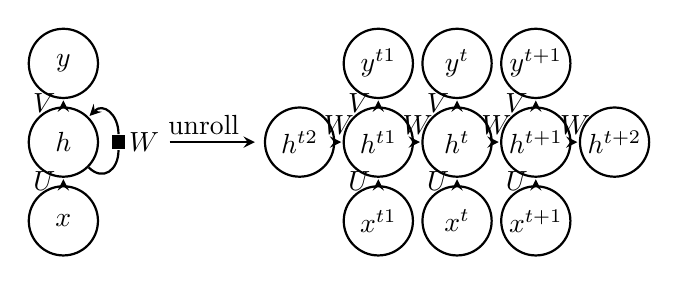
\begin{tikzpicture}[
    >=stealth, % default arrow style
    every node/.append style={inner sep=0.5pt},
    every path/.append style={-stealth, thick, shorten >=0.5pt}
]
\tikzstyle{place}=[circle, draw=black, minimum size=2.5em]

% --- "rolled" RNN ---

    \node[place] (y) at (0,2) {$\symbf y$};
    \node[place] (h) at (0,1) {$\symbf h$};
    \node[place] (x) at (0,0) {$\symbf x$};
    \draw (x) --node[left=2pt] {$\symbf U$} (h);
    \draw (h) --node[left=2pt] {$\symbf V$} (y);

    \node[fill=black,minimum size=0.5em] (W) at (0.7,1) {};
    \node[right=0cm and 0cm of W] {$\symbf W$};
    \draw (h) to[out=-45,in=-90,looseness=1.5] (W) to[out=90,in=45,looseness=1.5] (h);

% --- Rightarrow "unroll"

    \draw (1.35,1) --node[above=2pt] {unroll~~~} (2.45,1);

% --- unrolled RNN ---

    % all y's
    \node[place] (yt-1) at (4,2) {$\symbf y^{t\shortminus1}$};
    \node[place] (yt)   at (5,2) {$\symbf y^{t}$};
    \node[place] (yt+1) at (6,2) {$\symbf y^{t+1}$};
    % all h's
    \node[place] (ht-2) at (3,1) {$\symbf h^{t\shortminus2}$};
    \node[place] (ht-1) at (4,1) {$\symbf h^{t\shortminus1}$};
    \node[place] (ht)   at (5,1) {$\symbf h^{t}$};
    \node[place] (ht+1) at (6,1) {$\symbf h^{t+1}$};
    \node[place] (ht+2) at (7,1) {$\symbf h^{t+2}$};
    % all x's
    \node[place] (xt-1) at (4,0) {$\symbf x^{t\shortminus1}$};
    \node[place] (xt)   at (5,0) {$\symbf x^{t}$};
    \node[place] (xt+1) at (6,0) {$\symbf x^{t+1}$};

    % h-h connections (horizontal)
    \draw (ht-2) --node[above=2pt] {$\gray\symbf W$} (ht-1);
    \draw (ht-1) --node[above=2pt] {$\gray\symbf W$} (ht);
    \draw (ht)   --node[above=2pt] {$\gray\symbf W$} (ht+1);
    \draw (ht+1) --node[above=2pt] {$\gray\symbf W$} (ht+2);
    % x-h connections (vertical)
    \draw (xt-1) --node[left=2pt] {$\gray\symbf U$} (ht-1);
    \draw (xt)   --node[left=2pt] {$\gray\symbf U$} (ht);
    \draw (xt+1) --node[left=2pt] {$\gray\symbf U$} (ht+1);
    % h-y connections (vertical)
    \draw (ht-1) --node[left=2pt] {$\gray\symbf V$} (yt-1);
    \draw (ht)   --node[left=2pt] {$\gray\symbf V$} (yt);
    \draw (ht+1) --node[left=2pt] {$\gray\symbf V$} (yt+1);

\end{tikzpicture}
\end{scriptsize}

\end{figure}

\textbf{Backpropagation through time:}
\begin{itemize}
    \item Propagate derivates backwards through time
    \item Parameter sharing leads to a sum over $t$
    \item \textit{Def.} shortcut $\dot\sigma_i^t \coloneqq \sigma' (\bar F_i (h^{t\shortminus1}, x^t))$,\enskip $\symbf S(\symbf h^r) = \diag(\dot\sigma_1^r, {\ldots}, \dot\sigma_n^r)$
    \item \textbf{RNN gradients:} $\nabla_{\symbf x^t} \mathcal R = \brack*{\prod_{r=t+1}^s \symbf{W^\top S}(\symbf h^r)} \cdot \symbf J_H \cdot \nabla_{\symbf y} \mathcal R$
\end{itemize}


% ===
\subsection{Memory Units -- LSTM}

Classical RNNs easily forget (info gets ``washed out'').

\begin{figure}[H]
    \label{fig:lstm}
    \centering
    \begin{flushleft}
        \color{BlueViolet}\sffamily\scriptsize
        \quad (1): element-wise, to (not) pass information,\\
        \quad (2): add info to memory $C_t$
    \end{flushleft}\vspace{-2em}
    %! Author = tstreule

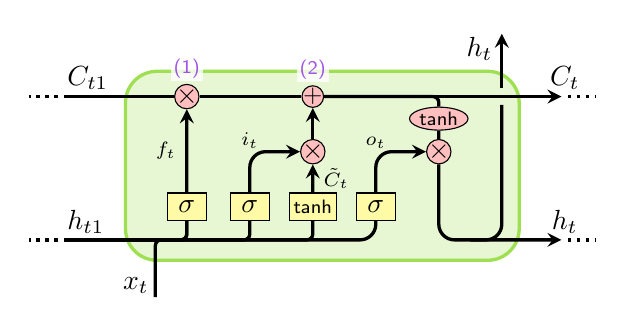
\begin{tikzpicture}[
    % Global config
    font=\sffamily,
    >=stealth, % default arrow style
    x=8mm,
    y=7mm,
    % Styles
    cell/.style={% the main box
        rectangle, rounded corners=4mm,
        draw=lime!70!teal!80, very thick,
        fill=lime!70!teal!20,
    },
    operator/.style={% operators like 'plus/+' or 'multiply/x'
        circle, inner sep=-.5pt,
        draw, fill=red!25,
    },
    function/.style={% functions like 'tanh'
        operator,% inherit style
        ellipse, inner sep=.5pt,
    },
    external/.style={% external in-/outputs
        inner sep=1pt,
    },
    knot/.style={% internal knots
        rectangle, inner sep=1.5pt,
        minimum width=5mm, minimum height=1em,
        draw, fill=yellow!35,
    },
    rigidArrow/.style={% arrows w/ tight corners
        rounded corners=.75mm,
        very thick,
    },
    roundArrow/.style={% arrows w/ big rounded corners
        rigidArrow,% inherit style
        rounded corners=2mm,
    },
    reference/.style={% text for reference
        rectangle, color=BlueViolet, fill=white, fill opacity=0.8,
        inner sep=1pt, outer sep=1pt,
    },
]

% Draw elements
    % Draw the cell / main box
    \node [cell, above right, minimum width=50mm, minimum height=24mm] at (0,0) {};

    % Draw internal knots --- knot-#
    \node [knot] (knot-1) at (1,1) {$\sigma$};
    \node [knot] (knot-2) at (2,1) {$\sigma$};
    \node [knot] (knot-3) at (3,1) {\scriptsize tanh};
    \node [knot] (knot-4) at (4,1) {$\sigma$};

    % Draw operators --- mul-# , sum-# , fct-#
    \newcommand{\myplus}{\scalebox{.9}{$+$}}
    \node [operator] (mul-1) at (1,3) {$\times$};
    \node [operator] (sum-1) at (3,3) {\myplus};
    \node [operator] (mul-2) at (3,2) {$\times$};
    \node [operator] (mul-3) at (5,2) {$\times$};
    \node [function] (fct-1) at (5,2.6) {\scriptsize tanh};
    \node [reference, above=0mm of mul-1] {\scriptsize(1)};
    \node [reference, above=0mm of sum-1] {\scriptsize(2)};

    % Draw inputs --- c-in , h-in, x
    \node [external] (c-in) at (-1,3) {};
    \node [external, above right=0pt and 0pt of c-in] {$C_{t\shortminus1}$};
    \node [external] (h-in) at (-1,.4) {};
    \node [external, above right=0pt and 0pt of h-in] {$h_{t\shortminus1}$};
    \node [external] (x) at (.5,-.7) {};
    \node [external, above left=0pt and 0pt of x] {$x_t$};

    % Draw outputs --- c-out , h-out , h-out2
    \node [external] (c-out) at (7,3) {};
    \node [external, above=0pt of c-out] {$C_t$};
    \node [external] (h-out) at (7,.4) {};
    \node [external, above=0pt of h-out] {$h_t$};
    \node [external] (h-out2) at (6,4.2) {};
    \node [external, below left=0pt and 1pt of h-out2] {$h_t$};

% Connect elements
    % dotted lines
    \draw [dotted, rigidArrow] (c-in) -- ++(-0.5,0);
    \draw [dotted, rigidArrow] (h-in) -- ++(-0.5,0);
    \draw [dotted, rigidArrow] (c-out) -- ++(0.5,0);
    \draw [dotted, rigidArrow] (h-out) -- ++(0.5,0);

    % inward connections
    \draw [->, rigidArrow] (c-in) -- (mul-1) -- (sum-1) -- (c-out);
    \draw [->, rigidArrow] (h-in) -| (knot-1) --node[left]{\scriptsize$f_t$} (mul-1);
    \draw [- , rigidArrow] (h-in) -| (knot-2);
    \draw [->, rigidArrow] (h-in) -| (knot-3) --node[right]{\scriptsize$\tilde C_t$} (mul-2);
    \draw [->, rigidArrow] (mul-2) -- (sum-1);
    \draw [->, roundArrow] (h-in) -| (knot-4) |-node[above=-1mm]{\scriptsize $o_t$} (mul-3);
    \draw [->, roundArrow] (knot-2) |-node[above=-1mm]{\scriptsize$i_t$} (mul-2);
    \draw [- , rigidArrow] (x) -- (x |- h-in) -| (knot-1);

    % outward connections
    \draw [- , rigidArrow] (sum-1) -| (fct-1) -- (mul-3);
    \draw [->, roundArrow] (mul-3) |- (h-out);
    \draw (c-out -| h-out2) ++(0,-0.15) coordinate (i1); % find intersection
    \draw [- , roundArrow] (h-out -| h-out2)++(-.5,0) -| (i1);
    \draw [->, roundArrow] (i1)++(0,0.3) -- (h-out2);

\end{tikzpicture}
%    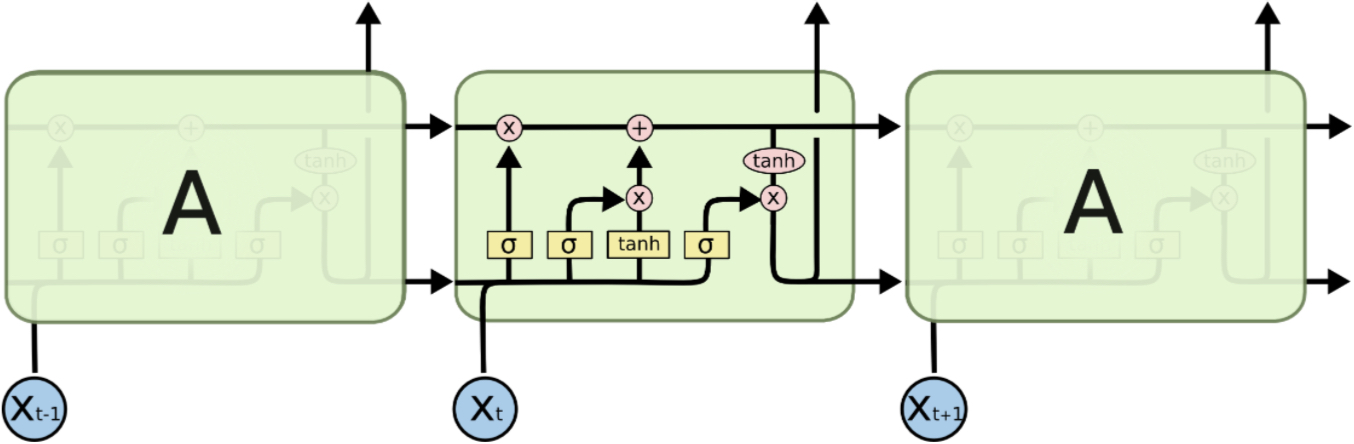
\includegraphics[width=.8\linewidth]{lstm_architecture}
\end{figure}

\begin{itemize}
    \item Information propagates along the chain
    \item can flow unchanged, only selectively changed by $\sigma$-gates
    \item can forget (when $f_t \approx 0$)
    \item LSTMs and GRUs can learn active memory strategies
    \item difficult to understand and resource-hungry
\end{itemize}


% ===
\subsection{Seq2Seq learning}

\textbf{Encoder RNN} $\symbf x \mapsto \symbf z$ and
\textbf{Decoder RNN} $\symbf z \mapsto \symbf y^{1:S}$ e.g. use encoder output as input for decoder and stop symbol \texttt{<EOS>}.

Can use Seq2Seq also for \textbf{image-to-text} sequencing, \ldots!


\textbf{Downsides of RNN:} (i) they don't work well for longer sequences, (ii) cannot be parallelized since architecture is sequential.

        %! Author = tstreule

\section{Deep Gradients}\label{sec:deep-gradients}


% ===
\subsection{Short connectivity}

\emph{Residual connections:}\enskip
shortcut layers and \textbf{add} back in,\enskip $g(\symbf x) = f(\symbf{x; \theta}) \green + \symbf x$, or if dimensions don't match: $f(\symbf{x; \theta}) \green + \symbf{Wx}$

\emph{Skip connections:}\enskip
shortcut layers and \textbf{concatenate} back in.
Connect layer output to all downstream layers.


% ===
\subsection{Normalization}

We observe \textbf{vanishing gradients}, i.e. poor backpropagation of errors, when incoming data to activation function is not normalized.


\subsubsection{Batch normalization \enskip\mdseries $\implies$ across many data points}

\begin{itemize}
    \item Learning rate $\eta$ is otherwise very sensitive
    \item Key idea: normalize the layer activation (and backpropagate through normalization!)
\end{itemize}
($+$) very effective, broadly used in vision\\
($-$) dependence on batch size, not suitable for all architectures


\subsubsection{Layer normalization \enskip\mdseries $\implies$ across units in same layer}

\begin{itemize}
    \item In scenarios like recurrent NNs, we have batch size = 1; batch normalization is not possible.
    \item Use population average of activations in layer as reference
\end{itemize}
($+$) very effective, used in NLP (transformers, RNNs)\\
($-$) no consistent benefits

        %! Author = tstreule

\section{Regularization}\label{sec:regularization}

\begin{formula}{Weight decay}
    L2-regularization;
    pulls weights towards zero.
\end{formula}

\begin{formula}{Early stopping}
    use validation data to estimate expected risk.\\
    $\to$ acts as approximate L2-regularizer!
\end{formula}

\begin{formula}{Bagging}
    combine models trained on bootstrap samples $S_r^k$.\\
    $\to$ almost always beneficial, but expensive!
\end{formula}

\begin{formula}{Dropout}
    randomly ``drop'' subsets of units in network.\\
    $\to$ each neuron learns to detect a feature that is \textit{generally} helpful!\enskip
    $\vert\to$ effectively defines an exponential \textbf{ensemble} w/o suffering the drawback of having to evaluate multiple layouts.
\end{formula}


% ===
\subsection{Data augmentation}

Exploit input \textbf{invariances} by generating virtual examples subject to transformations $\tau$ (highly domain specific).

\begin{formula}{Injecting noise}
    to inputs, weights and/or targets
\end{formula}


% ===
\subsection{Task augmentation}

\textbf{Pre-training:}\enskip
use pre-trained parts of the model. May also \textit{fine-tune} parameters.

\textbf{Semi-superivsed learning:}\enskip
optimize \textit{additive combination} of supervised and unsupervised risk, while \textbf{sharing parameters}.
$\to$ (typically) when more unlabeled that labeled data.

\textbf{Multitask learning:}\enskip
share (low level) representations across tasks and learn jointly.
$\to$ Learn high level repr. \textit{per task}.

        %! Author = tstreule

\section{Theory of DNNs}\label{sec:dnn-theory}


\emph{Consistency:}\enskip
\textbf{VC inequality:}\enskip
if worst-case empirical risk minimizer diverges, it will happen for the true case.


\emph{Spectral complexity:}\enskip
%for arbitraty ref. matrix $M^l$
%\begin{formula}
%    $R(\mathcal A) = \paren*{
%        \prod_{l=1}^L \rho^l \norm{W^l}_2
%    } \paren*{
%        \sum_{l=1}^L \frac{\norm{(W^l - M^l)^\top}_{2,1}^{2/3}}{\norm{W^l}_2^{2/3}}
%    }^{\raisebox{-3pt}{\math\scriptstyle3/2\endmath}}$
%\end{formula}
%For any margin $\gamma>0$ and probability $(1-\delta)$ over samples:
you can see the randomness of your data given the normalized margins!
\begin{formula}
    Test error$(f) \leq$ empirical $\gamma$-margin error$(f)$
\end{formula}


\emph{Double descent risk curves:}\enskip
DNNs contradict the classical view of bias-variance tradeoff.
\textit{Note:} this behavior is invisible when we use regularizers from the beginning.

        %! Author = tstreule

\section{Attention}\label{sec:attention}


\textbf{RNNs:}\enskip learn to encode information relevant for the future.\\
\textbf{Attention:}\enskip select what is relevant in retrospective.


% ===
\subsection{Self attention \enskip\mdseries($\symbf h_e^j$: encoder hidden state $j$)}

\begin{formula}*{Softmax Gating}
    $f_\phi (\symbf\xi, \symbf h_e^{1:s}) =
    \frac{1}{\sum_j \exp(\phi(j))}
    \begin{pmatrix}
        \exp(\phi(\symbf\xi, \symbf h_e^1)) \\[-0.3em]
        \vdots \\[-0.2em]
    \end{pmatrix}
    \gray \in \R^s$
\end{formula}
\begin{formula}{Gating function}
    Similarity or compatibility $\phi\colon \R^n \times \R^m \to \R$.
    $\to$ often an MLP, e.g. $\phi(\symbf\xi, \symbf h_3) = \symbf\xi \cdot \symbf h_e$ for $n {=} m$
\end{formula}

\begin{formula}*{Self-gated Attention}
    $\symbf z^{1:n} =
    [\symbf h_e^1, \ldots, \symbf h_e^s] \cdot f_\phi(\symbf\xi, \symbf h_e^{1:s})
    \gray \in \R^{n \times s} {\times} \R^{s}$
\end{formula}
\hfill$\to$ use those ``read-outs'' as input to the decoding RNN!


% ===
\subsection{Transformers}

Sequential nature of RNNs lead to \textit{memory limitations} and increased \textit{computation time}.
IDEA: Preserve attention, and encoder-decoder architecture, but\ldots

\begin{figure}[H]
    \label{fig:transformer}
    \centering
    %! Author = tstreule

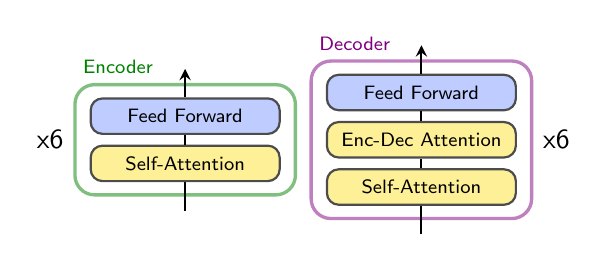
\begin{tikzpicture}[
    % Global config
    font=\sffamily\scriptsize,
    >=stealth, % default arrow style
    x=30mm,
    y=6mm,
    % Styles
    encdecbox/.style={% encoder and decoder box
        rectangle, rounded corners=2.5mm,
        very thick, minimum width=28mm,
    },
    basebox/.style={% base box for style inheritance
        rectangle, rounded corners=1.5mm,
        draw=black!70, thick,
        inner sep=1pt,
        minimum width=24mm, minimum height=4.5mm,
    },
    feedforward/.style={% feed forward box layer
        basebox, fill=blue!80!cyan!25,
    },
    attention/.style={% attention box layer
        basebox, fill=yellow!90!red!40,
    },
    arrow/.style={% arrow style
        thick,
    },
]

    \colorlet{encoder}{Green}
    \colorlet{decoder}{Purple}

% Draw elements
    % Encoder
    \node [encdecbox, draw=encoder!50, minimum height=14mm] (enc) at (0,0) {};
    \node [attention] (att-enc) at (0,-.5) {Self-Attention};
    \node [feedforward] (ff-enc) at (0,.5) {Feed Forward};
    \node [above left=2mm and 0mm of enc, anchor=west] {\color{encoder}Encoder};
    \node [left=0mm of enc, anchor=east] {\normalsize x6};

    % Decoder
    \node [encdecbox, draw=decoder!50, minimum height=20mm] (dec) at (1,0) {};
    \node [attention] (att-dec) at (1,-1) {Self-Attention};
    \node [attention] (att-enc-dec) at (1,0) {Enc-Dec Attention};
    \node [feedforward] (ff-dec) at (1,1) {Feed Forward};
    \node [above left=2mm and 0mm of dec, anchor=west] {\color{decoder}Decoder};
    \node [right=0mm of dec, anchor=west] {\normalsize x6};

% Connect elements
    \draw [->, arrow] (att-enc)++(0,-1) -- (att-enc) -- (ff-enc) -- ++(0,1);
    \draw [->, arrow] (att-dec)++(0,-1) -- (att-dec) -- (att-enc-dec) -- (ff-dec) -- ++(0,1);
%    \draw [<-, arrow] (att-enc) -- ++(0,-.8);
%    \draw [->, arrow] (att-enc) -- (ff-enc);
%    \draw [->, arrow] (ff-enc) -- ++(0,.8);

\end{tikzpicture}
\end{figure}

\textbf{Self attention:}\enskip
captures relations between words in a sentence. Use (query-key-value) word embeddings.
$\to$ think of it as a Google search / retrieval process\enskip
$\to$ can be computed in parallel!\enskip
Afterwards, use layer normalization.

\textbf{Enc-Dec attention:}\enskip
mimics attention mechanism of Seq2Seq models $\to$ input to output attention!\enskip

($+$) very powerful for solving encoder-decoder NLP problems\\
($-$) hard to train, attention results are not well interpretable


\subsubsection{Embedding from language models --- ELMO}

\textit{Bi}directional LSTM!\enskip
l2r for prediction,\enskip
r2l for context.


\subsubsection{Bidirect. Enc. Repr. from Transformers --- BERT}

Builds from \textit{ELMO} and \textit{GPT} but is a \textbf{few-shot learner}.
Compared to traditional \textit{fine-tuning}, this shows that such large NLP models have \textbf{learnt to learn}.

        %! Author = tstreule

\section{Variational Autoencoders}\label{sec:vae}


\begin{formula}{Define}
    $\xrightarrow[\text{prior}]{p_{\theta'}(z)} \mathcal Z
    \xrightarrow[\text{likelihood}]{\mathrm{dec}_\theta(z) = p_\theta(x\mid z)} \mathcal X
    \xrightarrow[\text{approx. posterior}]{\mathrm{enc}_\phi(x) = q_\phi(z\mid x)} \mathcal Z$
    \\ $\to$ sample/observe $\mathcal X_i$ from latent representation $\mathcal Z$
\end{formula}

\newcommand\getcolor{\colorlet{previousColor}{.}}
\newcommand\resetcolor{\color{previousColor}}

\begin{formula}{Train}
    $\max\limits_{\theta', \theta, \phi} \sum_{i} \getcolor\orange\underbracket{{\resetcolor \log p_{\theta', \theta} (x_i)}}\nolimits_{\ (\ast) \text{ indep. of } Z}$
    \\
    \begin{tabular}{r@{~}l}
        $\orange{(\ast)} =$
        & $\E*[Z \sim q_\phi(\cdot \mid x_i)]{\log\paren*{ \frac{p_{\theta', \theta}(x_i, Z)}{p_{\theta', 'theta}(Z \vert x_i)} \ \frac{q_\phi(Z \vert x_i)}{q_\phi(Z \vert x_i)} }}$
        \\
        $=$ & $\overbracket{
            \E*{\log p_\theta(x_i\mid Z)}
            - D\ped{KL}\paren*{q_\phi(\cdot\mid x_i) \parallel p_{\theta'}(\cdot)}
        }^{\begingroup\color{Green} \mathcal L(x_i,\theta,\phi) \endgroup \:\equiv\: \text{\textbf{ELBO} = Infomax -- Regularisation term}}$
        \\
        & $+ D\ped{KL}\paren*{q_\phi(\cdot\mid x_i) \parallel p_{\theta', \theta}(\cdot\mid x_i)}
        \color{Green} \geq \mathcal L(x_i, \theta, \phi)$
    \end{tabular}
    \\
    $\implies$ \highlight{$\theta^\ast, \phi^\ast = \arg\max_{\theta,\phi} \mathcal L(x_i, \theta, \phi)$}
\end{formula}

Requirements for good representation:
\begin{itemize}
    \item \textbf{informative:}\enskip
    $\theta^\ast = \arg\max_\theta I(X;Z)
    \gray{= \arg\max_\theta \E[X,Z]{\log p(X\mid Z)} - \textit{const}_{\textit{w.r.t. } \theta}}
    \approx \arg\max_\theta \sum_i \E[Z\mid X]{\log p(x_i\mid Z)}$
    \item \textbf{disentangled:}\enskip
    components in $\mathcal Z$ associated with distinct feature in $\mathcal X$
    (see $D\ped{KL}$ in ELBO).
    \item \textbf{robust:}\enskip
    noise in $\mathcal Z$ doesn't substantially affect $\mathcal X$ (and vice versa)
    $\to$ choice of approx. posterior!
\end{itemize}

        %! Author = tstreule

\section{Adversarial Robustness}\label{sec:adversarial-robustness}


How to measure robustness of linear, \textbf{binary} classifier?
$\arg\min_r \norm{r}_p$ s.t. $f_1(x+r) - f_2(x+r) < 0$.

For $p=2$: $r_i=\frac{f_1(x)-f_2(x)}{\norm{w_2 - w_1}} (w_2 - w_1)$.
\enskip
\textbf{Multi-class} case:\\ $\arg\min_{\brace{r_i}} \norm{r_i}_2$
$\leftarrow$ pick min. distance from $x$ to any polytope.


\textbf{IDEA:}\enskip Improve robustness through adversarial training!
%\begin{formula}{$\ell_p$-norm robustness}
%    $k(x+r) \approx k(x)$ for small $\norm{r}_p$
%\end{formula}
\begin{formula}*{Standard train loss}
    $\min_\theta \ell(f_\theta(x), y)$
\end{formula}
\begin{formula}*{$L_p$-robust train loss}
    $\min_\theta \max_{\norm{r}_p \leq \epsilon} \ell(f_\theta(x+r), y)$
\end{formula}
\begin{formula}
    Project gradient \textbf{ascent} via
    $r \mapsto
    \begin{cases}
         r_i & \abs{r_i} \leq \epsilon \\
         \epsilon & \text{otw.}
    \end{cases}
    \leq \epsilon \cdot \sign(r_i)$
\end{formula}
        %! Author = tstreule

%\vfill~\columnbreak

\section*{Appendix}\label{sec:appendix}


\begin{formula}{Taylor}
    \highlight{$f(\symbf x + \Delta\symbf x) \approx f(\symbf x) + \nabla f(\symbf x)^\top \Delta\symbf x + \frac12 \Delta\symbf x^\top \nabla^2 f(\symbf x) \Delta\symbf x$}
\end{formula}
\begin{formula}{Cauchy-Schwarz}
    $\abs*{\E{X,Y}}^2 \leq \E{X^2} \E{Y^2}$
\end{formula}
\begin{formula}{Jensen, {\mdseries $f(~\cdot~)$ convex}}
    $f(\E{x}) \leq \E{f(X)}$
\end{formula}

\begin{formula}{Derivative}
    $\nabla_{\symbf v} f(\symbf w) = \nabla f(\symbf w)^\top \symbf v = \lim\limits_{\lambda\to0} \frac{f(\symbf w + \lambda \symbf v) - f(\symbf w)}{\lambda}$
\end{formula}


% ===
\subsection*{Probability / statistics}

\begin{itemize}
    \item Gaussian:
    $\Gauss{x \mid \mu, \sigma^2} = \frac{1}{\sqrt{2\pi\sigma^2}} \exp*(-\frac12 \frac{(x-\mu)^2}{\sigma^2})$
    \\
    $\Gauss{\symbf{x \mid \mu, \Sigma}} = \frac{1}{\sqrt{(2\pi)^d \abs{\symbf\Sigma}}} \exp*(-\frac{1}{2} (\symbf x - \mu)^\top \symbf \Sigma^{\shortminus1} (\symbf x - \mu))$
    % \\
    % $\ln(\Gauss{}) {=} {-} \frac{\ln\abs{\symbf\Sigma}}{2} {-} \frac12 (\symbf x{-}\symbf\mu)\!^\top \symbf\Sigma^{-1} (\symbf x{-}\symbf\mu) + const$%{-} \frac{d}{2} \ln(2\pi)
    \\
    $X \sim \Gauss{\symbf{\mu, \Sigma}}$,\enskip $Y = A {+} BX \implies Y{\sim}\Gauss{A {+} B \symbf\mu,\ B \symbf\Sigma B\!^\top}$
    \item Binom.: $f(k,n;p) = \P{X=k} = \binom nk p^k (1-p)^{n-k}$
    \item $\V{X} = \E{(X - \E{X})^2} = \E{X^2} - \E{X}^2$ \\
    $\V{X+Y} = \V{X} + \V{Y} + 2\Cov{X,Y}$
    \item $\Cov{X,Y} = \E{(X-\E{X})(Y-\E{Y})} = \E{XY} - \E{X}\E{Y}$ \\
    $\Cov{aX,bY} = ab\Cov{X,Y}$
\end{itemize}

\emph{Complete the square:}\\
If $p(\symbf x) \propto \exp(-\frac12 \symbf x^\top \symbf{\orange{A}x} + \symbf x^\top \orange{\symbf b})$,
then $p(\symbf x) = \Gauss{\symbf x \mid \symbf A^{\shortminus1} \symbf b, \symbf A^{\shortminus1}}$

\emph{Conditional Gaussians:}\enskip
$\implies Y\vert X \sim \Gauss{\tilde{\symbf\mu}, \tilde{\symbf\Sigma}}$,\enskip where\\
$\tilde{\symbf\mu} = \symbf\mu_Y + \symbf\Sigma_{YX} \symbf\Sigma_{XX}^{\shortminus1} (X - \symbf\mu_X)$,\enskip
$\tilde{\symbf\Sigma} = \symbf\Sigma_{YY} - \symbf\Sigma_{YX} \symbf\Sigma_{XX}^{\shortminus1} \symbf\Sigma_{XY})$\\
$P_{X,Y} = \begin{bmatrix} \symbf X \\ \symbf Y \end{bmatrix} \sim
\Gauss*[~]{
    \begin{bmatrix} \symbf\mu_X \\ \symbf\mu_Y \end{bmatrix} ,
    \begin{bmatrix} \symbf\Sigma_{XX} & \symbf\Sigma_{XY} \\ \symbf\Sigma_{YX} & \symbf\Sigma_{YY} \end{bmatrix}
}$,\enspace $\symbf\Sigma_{ij}$ p.s.d.


% ===
\subsection*{Calculus}

\begin{formula}
    \raggedright
    \newcommand{\Item}[1]{\textbullet\nobreak\enskip#1\hfill\enskip\allowbreak}
    \newcommand{\Tr}{\mathop{T\!r}}
    \Item{$\int_a^b u v' \diff x = u v \vert_a^b - \int_a^b u' v \diff x$}
    \Item{$\pderiv{x} \frac{g}{h} = \frac{g'h}{h^2} - \frac{gh'}{h^2}$}
    \Item{$\pderiv{\symbf x} f(\symbf x) = \diag (f'(\symbf x))$}
    \Item{$\pderiv{\symbf x} (\symbf b^\top\symbf  x) = \pderiv{}{\symbf x} (\symbf x^\top\symbf  b) = \symbf b$}
    \Item{$\pderiv{\symbf x} (\symbf b^\top \symbf{Ax}) = \symbf A^\top \symbf b$}
    \Item{$\pderiv{\symbf x} (\symbf x^\top \symbf{Ax}) = (\symbf A^\top + \symbf A)\symbf x \overset{\orange{\ast}}{=} 2\symbf{Ax}$ \enskip \mbox{\gray\footnotesize $(\ast)$: $\symbf A$ sym.}}
    \Item{$\pderiv{\symbf X} (\symbf c^\top \symbf{Xb}) = \symbf{cb}^\top$}
    \Item{$\pderiv{\symbf X} (\symbf c^\top \symbf X^\top \symbf b) = \symbf{bc}^\top$}
    \Item{Trace trick: $\symbf{x^\top A x} \overset{\orange{\ast}}{=} \Tr(\symbf{x^\top A x}) \overset{\orange{\ast\ast}}{=} \Tr(\symbf{x x^\top A}) = \Tr(\symbf{A x x^\top})$ \enskip \mbox{\gray\footnotesize $(\ast)$: inner prod., $(\ast\ast)$: cyclic permut.}}
    \Item{$\pderiv{\symbf X} \Tr(\symbf{X^\top A}) = \symbf A$}
    \Item{$\abs{\symbf X^{\shortminus1}} = \abs{\symbf X}^{\shortminus1}$}
    \Item{$\pderiv{}{\symbf X} \log \abs{\symbf X} = \symbf X^{\shortminustop}$}
    \Item{$\deriv{}{x} \abs x = \frac{x}{\abs x}$}
    \Item{$\pderiv{}{\symbf x} \norm{\symbf x}_2 = \pderiv{}{\symbf x} (\symbf x^\top \symbf x) = 2\symbf x$}
    \Item{$\pderiv{}{\symbf x} \norm{\symbf x - \symbf b}_2 = \frac{\symbf x-\symbf b}{\norm{\symbf x-\symbf b}_2}$}
    \Item{$\pderiv{}{\symbf x} \norm{\symbf x}_1 = \sign(\symbf x)$ \enskip \mbox{\gray\footnotesize $\sign(\symbf x) \in \brace{\pm1}^p$ is row-wise}}
\end{formula}


%\vfill
%\todo{Links to review
%\begin{itemize}
%    \item \href{https://distill.pub/2017/momentum/}{Blog post about \textbf{momentum}}
%    \item \href{https://jalammar.github.io/visualizing-neural-machine-translation-mechanics-of-seq2seq-models-with-attention/}{Blog post about \textbf{attention}}
%    \item \textbf{(Vaswani et al. 2017)} ``Attention is all you need''
%\end{itemize}}


%        %! Author = tstreule

\section{Test document}\label{sec:test-document}


\subsection{Subsection}
\subsubsection{Subsubsection 1}
\subsubsection{Subsubsection 2 that has a ``g''}
\subsubsection{This is an annoingly, really, really, really long Subsubsection and some People may say it'll never end}


\subsection{Text}

Lorem ipsum

Lorem ipsum dolor sit amet, consetetur sadipscing elitr, sed diam nonumy eirmod tempor invidunt ut labore et dolore magna aliquyam erat, sed diam voluptua. At vero eos et accusam et justo duo dolores et ea rebum.

{\sffamily Lorem ipsum dolor sit amet, consetetur sadipscing elitr, sed diam nonumy eirmod tempor invidunt ut labore et dolore magna aliquyam erat, sed diam voluptua. At vero eos et accusam et justo duo dolores et ea rebum.}


\subsection{Tabular}

\begin{tabular}{llll}
    \rmfamily Serif & \rmfamily\itshape Italics
    & \rmfamily\bfseries Bold & \rmfamily\itshape\bfseries Bold italics
    \\
    \sffamily Sans-serif & \sffamily\itshape Italics
    & \sffamily\bfseries Bold & \sffamily\itshape\bfseries Bold italics
    \\
    \ttfamily Typewriter & \ttfamily\itshape Italics
    & \ttfamily\bfseries Bold & \ttfamily\itshape\bfseries Bold italics
\end{tabular}


\subsection{Itemize / enumerate}

\begin{itemize}
    \item Item 1
    \item Item 2
\end{itemize}
\begin{enumerate}
    \item Item 1
    \item Item 2\\\ldots
    \item[$\vdots$]
    \item[10.] Item 10
\end{enumerate}
asdf


\subsection{Math}

Textstyle: $\sum_{i=1}^\infty \frac1n$

Displaystyle: $\displaystyle\sum_{i=1}^\infty \frac1n$

And now an equation ...
\begin{equation*}
    Blah
\end{equation*}
... is encapsuled in this text.

\vfill~\columnbreak


$\overset{asdf}{fds}$

\section{blah}

\section{blah}

\begin{highlightbox}*
    This is a \texttt{highlightbox}
\end{highlightbox}

\begin{formula}
    Joe mama
\end{formula}
\begin{formula}{Test}
    $$\Re$$
\end{formula}

$\P*{\dfrac12}$

$\Gauss*{\dfrac12}$

$\Gauss d$
\\


$10\tothe{-4}$

%        ~\vfill\parbox{\linewidth}{\hrule\medskip\hrulefill\centering\textbf{ max. 4 A4-pages! }\hrulefill}

    \end{multicols*}
\end{document}
